\documentclass{../../../lessonplan}
\renewcommand{\cflroot}{../../..}

\begin{document}

\lessonplantitle
    {UKS2-S2}
    {Upper Key Stage 2 - Session 2}
    {Breaking down the problem into chunks (understanding procedures)}

\preamble
    {
    \item Decompose the programming task into smaller parts
    \item Identify sections of code which can be used several times and write a \keyword{procedure} for that section
    \item Use \keyword{repeat} loops within \keyword{procedures}
    }
    {
    \item Interactive White Board (IWB)
    \item Levels 61 to 67 in Rapid Router
    \item Resource sheets UKS2-S1-1 -- UKS2-S2-2
    \item UKS2 Levels Guide
    \item UKS2 Program Solutions Table
    \item UKS2 Assets - Blockly cards
    }
    {
    \item Procedure
    \item Decompose
    \item Define a procedure
    \item Call a procedure
    }

\begin{lessonplan}

Explain to pupils/to the class that often in programming we need to do the same task at different times in the program.

We can write the code for this task or \keyword{procedure} and give it a name.

Then we can \keyword{call} the \keyword{procedure} and give it a name.

\keyquestion{Let's think about familiar situations where we are actually using} \keyword{procedures}.

When a teacher says \textbf{``stop''} in class, what she actuall means is ``stop talking, pencil down and face the front''.
This is a set of instructions contained in the command \textbf{``stop''}.
Sot that command is like a mini-program which we call a procedure.
A teacher might use it several times in a lesson.

Another way of think about \keyword{procedures} is to look at verses which are used several times in a song or poem.
Talk about songs and stories where you need to use the same words or lyrics at different points. \textit{[fig S2.1]}

Watch the video of Michael Rosen performing `We're going on a Bear Hunt'.
Most children will be very familiar with this, but you could use a similar story/poem with familiar verses used in different stages of the narrative.

\fig{fig S2.1}{figS2.1.jpg}{1}

\url{http://www.youtube.com/watch?v=0gyI6ykDwds} or \url{http://www.youtube.com/ watch?v=ytc0U2WAz4s}

\keyquestion{Can you spot which sets of lines are used more than once in different parts of the story?}

They should find two obvious chunks: \\
\textbf{
`We're going on a bear hunt \\
We're going to catch a big one\\
What a beautiful day\\
We're not scared\\
Uh-oh'
}

Then: \\
\textbf{
`We can't go over it\\
We can't go under it\\
Oh no! \\
We've got to go through it!''
}

Resource sheet UKS2-S2-1 has each `chunk of lines' marked \keyword{procedure} 1 -- bear hunt and \keyword{procedure} -- over and under \textit{[fig S2.2]}

\fig{fig S2.2}{figS2.2.jpg}{1}


Give \keyword{procedure} 1 to one group of four children and \keyword{procedure} 2 to another group of four.

Show the rest of the class the story structure on the IWB, explaining that they will perform the parts not covered by the \keyword{procedures}.

Ask the class to perform the poem, calling each group to perform \keyword{procedure} 1 and \keyword{procedure} 1 as needed.

Recap the concept of a \keyword{procedure} just being a set of instructions which you name, and can be `\keyword{called}' in a program at any time.
Some children may hae spotted some \keyword{repeat} loops in the story e.g.\ Repeat 3 (swishy swashy).

Return to Rapid Router Level 61 on the IWB. \textit{[fig S2.3]}

\fig{fig S2.3}{figS2.3.jpg}{1}


Explain that the block of code to create a \keyword{procedure} is \keyword{Define} followed by the name you are giving to your \keyword{procedure}:

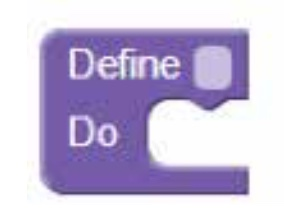
\includegraphics[width=.3\linewidth]{define.jpg}

In your program, when you want to use that \keyword{procedure}, the block of code is \keyword{Call}:


\includegraphics[width=.3\linewidth]{call.jpg}

Give each group a copy of the level screen from the levels guide.
Ask the children to come up with a solution with their talk partners to create a \keyword{procedure} for the wiggle in the road.

Make a note of the different solutions on a flipchart.
The following is the `model solution'---the most efficient.
Show this on the IWB and ask the children to check that it works and to compare it with their own solutions.

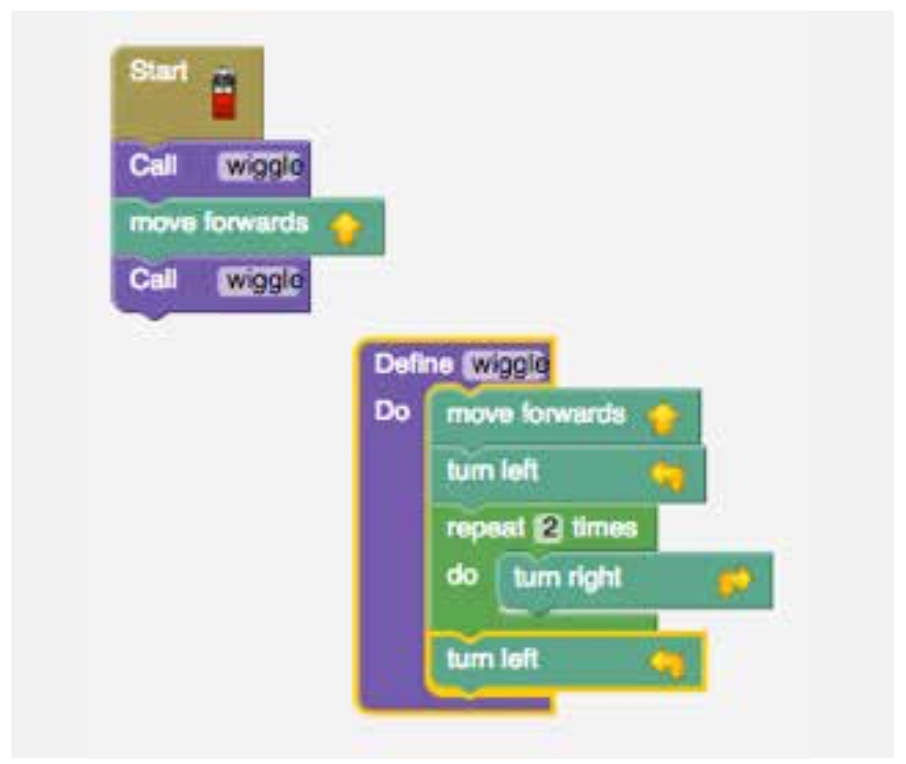
\includegraphics[width=\linewidth]{model.jpg}

\section*{Paired activity}

Children can try Levels 61 to 67 at their own pace, if you select similar ability pairs.

Alternatively, you may wish to start the activity off in mixed groups, to support those who find the concept challenging.

Ask them to work in pairs and use Resource Sheet UKS2-S2-2 to design their program before creating the code on screen.
Copies of the levels screenshots from the Levels Guide will be useful for some children.
If you wish, you could do this as an unplugged activity before using the computers. \textit{[fig S2.4]}

\fig{fig S2.4}{figS2.4.jpg}{1}

This will help children discuss their thought processing and support the debugging if needed.

\end{lessonplan}

\end{document}
